\documentclass[12pt]{article}

% Packages for double-spacing
\usepackage{setspace}
\usepackage{graphicx}
\doublespacing

\begin{document}

% Title and author information
\title{Graph Neural Network Model}

\maketitle

% Abstract
\begin{abstract}
    A  remarkable  number  of  ideas  across  various  domains  can be effectively
    depicted   as   graphs,  ranging  from  social  networks  and  railway  maps  to
    molecules.  Graphs  offer  an  elegant  way  to  abstract these concepts, making
    them   a   primary  tool  for  representing  data.  This  abstraction  not  only
    highlights  the  characteristics  of  individual  data  points but also captures
    the  relationships  between  them.  However,  this versatility poses a challenge
    in  the  field  of  machine  learning,  as  desining algorithms that efficiently
    handle such interconnected data has proven to be a challenging task.
\end{abstract}

% Introduction
\section{Introduction}
    We shall start by giving a brief introduction to out mathematical model.
    A graph $G$ is a pair $(V, E)$, where $V$ is the set of vertices, and 
    $E \subseteq V \times V$ is the set of edges, representing the relationships
    between the vertices.

    \begin{figure}
        \centering
        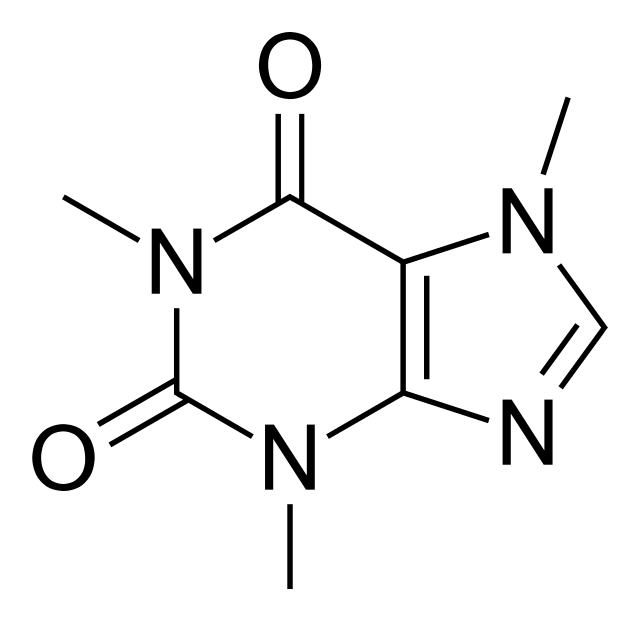
\includegraphics[width=0.4\textwidth]{img/Caffeine_structure.png}
        \caption{A molecule of caffeine, represented as a graph, where the vertices are the atoms and the edges are the bonds between them.}
        \label{fig:graph}
    \end{figure}

% Methodology
\section{Methodology}
This is the methodology section of your article.

% Results
\section{Results}
This is the results section of your article.

% Conclusion
\section{Conclusion}
This is the conclusion section of your article.

% References
\begin{thebibliography}{9}
\bibitem{reference1}
Author, A. (Year). Title of the reference.

\bibitem{reference2}
Author, B. (Year). Title of the reference.
\end{thebibliography}

\end{document}


